% Chapter Template

\chapter{Simulation} % Main chapter title

\noindent\textbf{\large Contents:}

\noindent\hrulefill
\noindent\startcontents[chapters]
\noindent\printcontents[chapters]{}{1}{}
\noindent\hrulefill

\label{Chapter2} % Change X to a consecutive number; for referencing this chapter elsewhere, use \ref{ChapterX}




\section{Response Matrix}

At the beginning of this project I was given two files, both of which were representative of the GMT pupil.  One was a binary amplitude mask of the GMT pupil and the other was the phase mask of the 

\begin{figure}[H]
\centering
\begin{subfigure}{.5\textwidth}
  \centering
  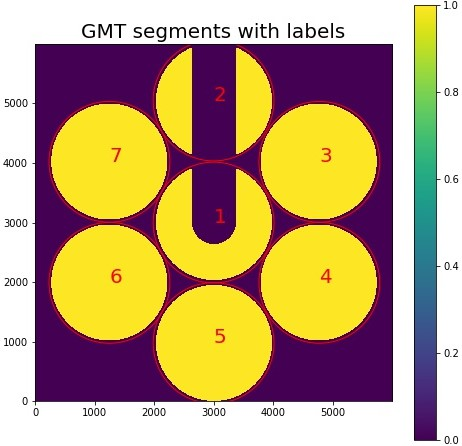
\includegraphics[width=10cm]{Figures/GMT_seg_choice.jpg}
  \caption{Amplitude mask of the GMT pupil.  Each segment is labeled 1-7 for which segment is to be isolated by the code.}
  \label{fig:sub1}
\end{subfigure}%
\begin{subfigure}{.5\textwidth}
  \centering
  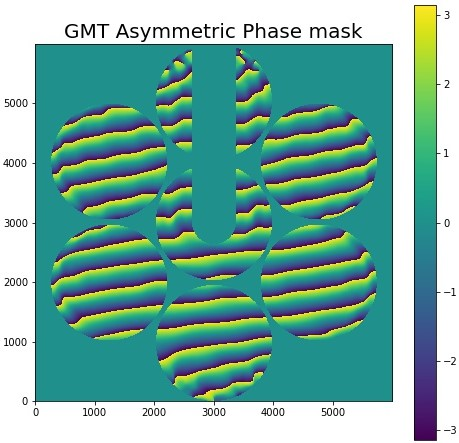
\includegraphics[width=12cm]{Figures/gmt_phase_mask.jpg}
  \caption{A subfigure}
  \label{fig:sub2}
\end{subfigure}
\caption{A figure with two subfigures}
\label{fig:test}
\end{figure}


\section{Control Matrix}



Mostly theoretically

\begin{itemize}
    \item GMT masks
    \item Singular values
    \item Building RM
    \item CM
\end{itemize}